\documentclass{article}
\usepackage[utf8]{inputenc}
\usepackage{float}
\usepackage{graphicx}
\usepackage{listings}
\usepackage{color}
\usepackage{textcomp} % straight single quotes
\usepackage{comment}
\usepackage[T1]{fontenc}
\newcommand\amelia[0]{\textsc{Amelia}}



% ====================================================================
% configuration for Pascani and Amelia listings
\definecolor{keywords}{RGB}{127,0,85}
\definecolor{comments}{RGB}{63,127,95}
\definecolor{strings}{RGB}{42,0,255}
\definecolor{frame}{RGB}{230,230,230}
\definecolor{numbers}{RGB}{160,160,160}
\lstdefinestyle{common}{
  tabsize=3,
  morestring=[b]',
  captionpos=b,
  showspaces=false,
  showtabs=false,
  breaklines=true,
  showstringspaces=false,
  breakatwhitespace=true,
  escapeinside={(*@}{@*)},
  commentstyle=\color{comments},
  keywordstyle=\bfseries\color{keywords},
  stringstyle=\color{strings},
  basicstyle=\small\ttfamily,
  frame=lines,
  rulecolor=\color{frame},
  xleftmargin=2em,
  framexleftmargin=1.5em,
  numbers=left,
  numbersep=6pt,
  numberstyle=\small\ttfamily\color{numbers}
}
\lstdefinestyle{pascani}{
  style=common,
  language=Java,
  morestring=[b]`,
  morekeywords={
    above,
    and,
    as,
    below,
    change,
    config,
    equal,
    event,
    exception,
    extension,
    from,
    handler,
    invoke,
    monitor,
    namespace,
    of,
    on,
    or,
    periodically,
    raised,
    to,
    using,
    val,
    var
  }
}

\lstdefinestyle{amelia}{
  style=common,
  language=Java,
  upquote=true, % straight single quotes
  literate={»}{}0{«}{}0,
  morekeywords={
    as,
    cd,
    cmd,
    compile,
    config,
    depends,
    deployment,
    eval,
    extension,
    includes,
    on,
    param,
    run,
    scp,
    subsystem,
    to,
    val,
    var
  }
}

\lstdefinestyle{xtext}{
  style=common,
  morecomment=[l]{//},
  morecomment=[s]{/*}{*/},
  morestring=[b]",
  upquote=true, % straight single quotes
  morekeywords={
    grammar,
    with,
    generate,
    import,
    as,
    returns,
    current,
    terminal
  }
}

% ====================================================================

\title{A Practical Guide to Amelia: A Domain Specific Language for Automated Software Deployment}
\author{ }
\date{October 2017}

\begin{document}

\maketitle

\section{Introduction}

To facilitate and promote the use of the \amelia{} DSL, our language that assists application developers in automating the deployment of component-based software systems, we designed a deployment case study to use the main features of \amelia{}. Through this practical guide, a \textit{software deployer} will be able to get a deeper understanding of the constructs defined in \amelia{}, which will increase the deployer's ability for specifying the required deployment specifications with the language.


\section{Case Study: The Matrix-Chain Multiplication Problem}

The Matrix-Chain Multiplication (MCM) problem is an optimization problem that consists in finding the most efficient multiplication sequence to multiply a set of given matrices. Our implementation of the MCM, provided to the workshop participants, splits the problem into three different subproblems: the matrix-pair multiplication problem, the matrix-chain parenthesization problem, which finds the optimal sequence of matrix-pair multiplications minimizing the number of individual additions and multiplications, and the matrix-subchain multiplication scheduling problem, which finds subsets of matrix multiplications that can be performed concurrently to decrease the overall multiplication time \cite{lee2003}. In this way, by combining the different solutions to these subproblems, it is possible to configure several different actual solutions to the whole problem, which raises a problem of solution configuration. For instance, by combining the first and second subproblems, one can obtain a solution able to multiply a set of given matrices reducing the number of individual arithmetical operations. In the same sense, by combining the first and third subproblems, one would obtain the same solution aforementioned, but this time reducing multiplication time. And of course, by combining the three subproblems one would reduce both operations and overall processing time. In practice, however, there can be computational limitations and trade-offs that may make infeasible some of the possible solution configurations. \\

\begin{figure}[H]
	\centering
	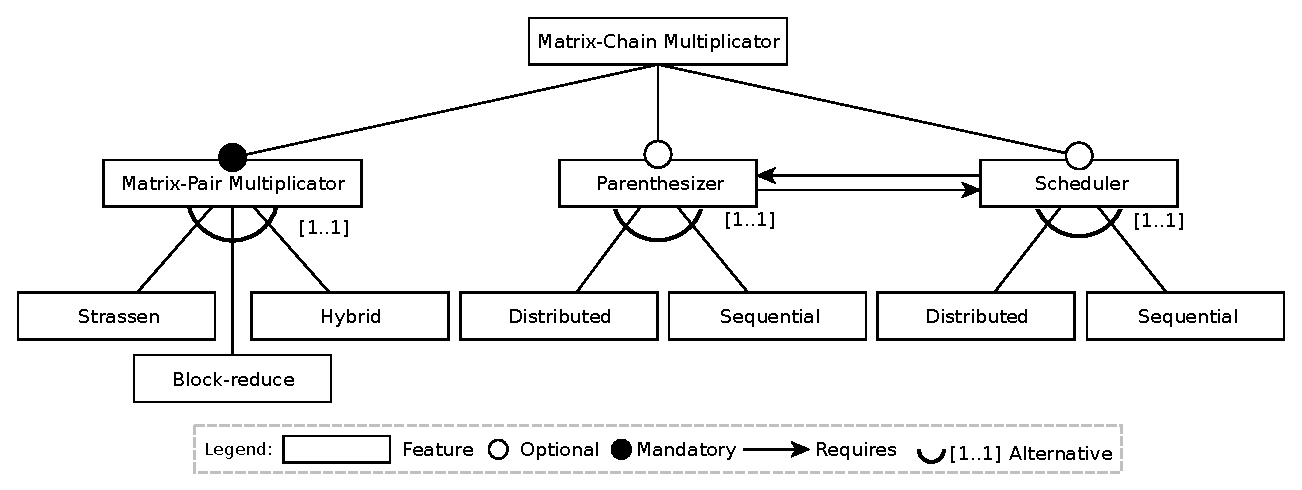
\includegraphics[width=5.5in,height=2.5in]{fig/evaluation/features-diagram}
\end{figure}

In this implementation of the MCM solution, we take advantage of distributed computational resources in order to reduce the execution time when multiplying a large number of considerably big matrices. To this end, we developed two multiplication strategies, one based on the map-reduce architecture, and a variation of it that significantly reduces network usage. At the end, local multiplications are performed using the Strassen algorithm. \\

The following deployment diagrams depict the high-level elements composing each of the multiplication strategies. For sake of simplicity, we omit the details of the scheduling and parenthesizing subproblems. As there is only one artifact per strategy (\textit{i.e.}, one resulting artifact of the compilation process), a note on each diagram specifies the node in which the components are executed. \\

%%%%%%%%%%%%%%%
\begin{comment}

\begin{figure}[H]
	\centering
	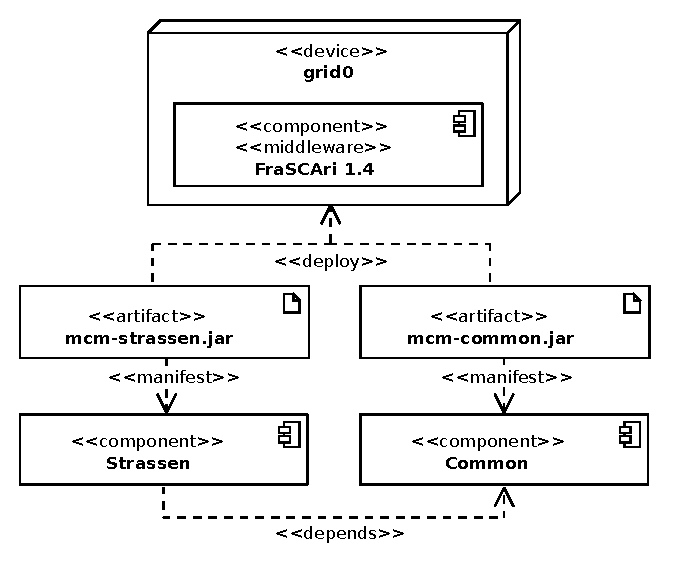
\includegraphics[width=0.6\textwidth]{fig/evaluation/strassen-deployment}
	\caption[]{Deployment Diagram for the Monolithic Strassen Configuration Strategy}
	\label{fig:apx-eval-amelia-strassen}
\end{figure}

The monolithic Strassen configuration strategy considers only a multiplication component that takes the sequence of matrices as it is, and multiplies them iteratively in one computing node. This strategy leaves out the optimizations introduced by subproblems matrix-chain parenthesization and matrix-subchain multiplication scheduling.
\end{comment}
%%%%%%%%%%%%%%%

\subsection{BlockReduce Strategy}

\begin{figure}[H]
	\centering
	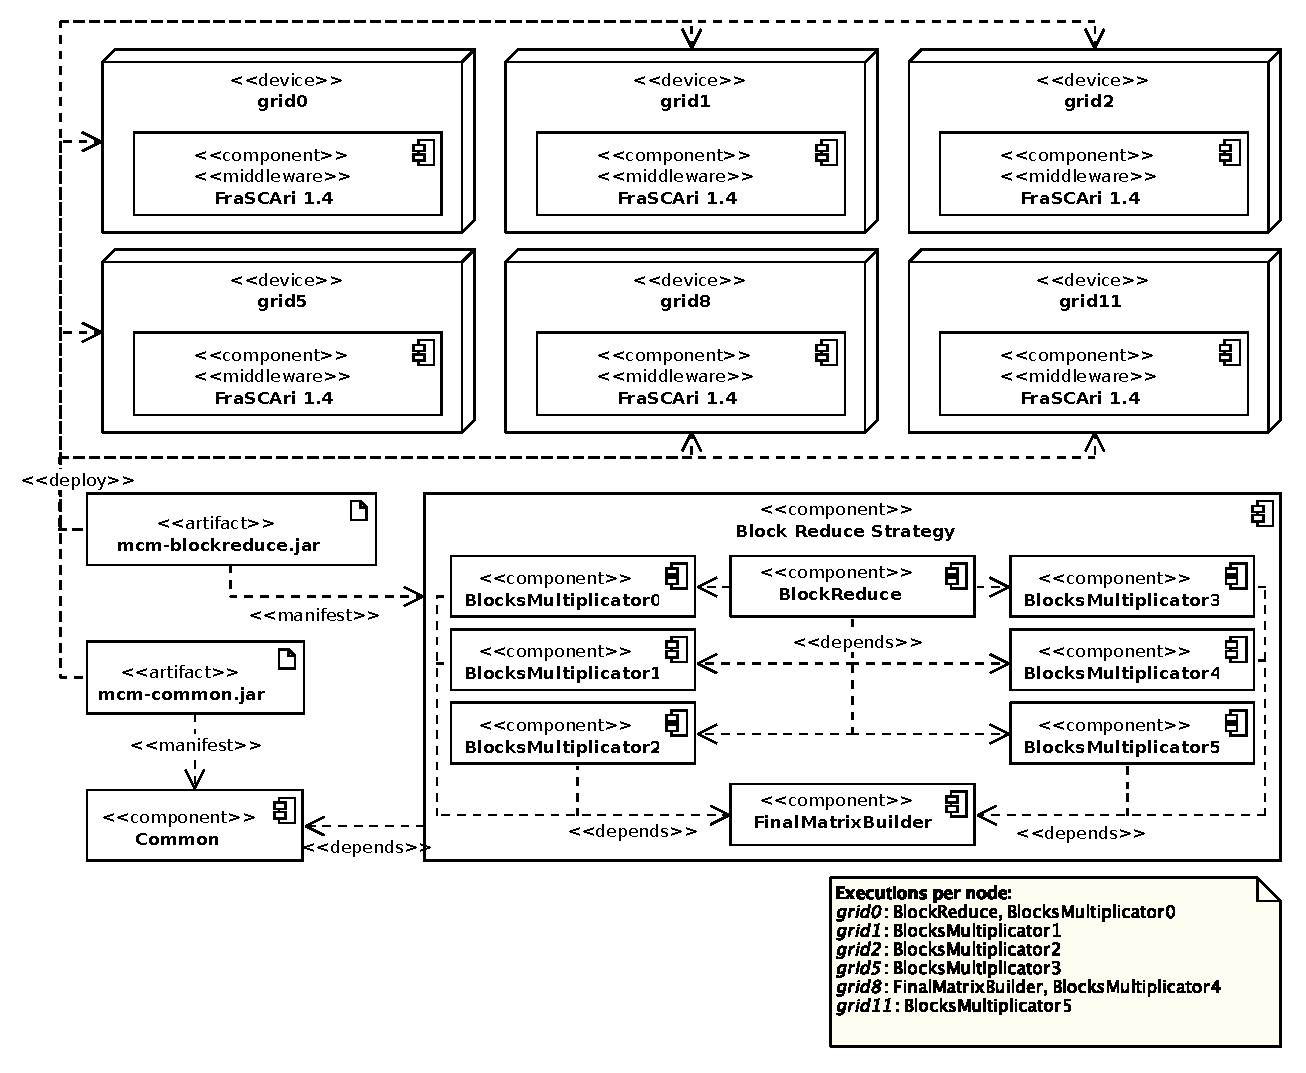
\includegraphics[width=0.8\textwidth]{fig/evaluation/blockreduce-deployment}
	\caption[]{Deployment Diagram for the BlockReduce Configuration Strategy}
	\label{fig:apx-eval-amelia-blockreduce}
\end{figure}

The BlockReduce consiguration strategy consists in splitting each matrix into fixed-size blocks (\textit{i.e.}, sub-matrices) and multiply them as if they were one cell instead of a group of them. For instance, having two squared matrices $A$ and $B$, partitioned into 4 blocks each, the resulting matrix $C$ would be calculated using the same blocks partition strategy. $C_{00}$ represents the first block of $C$, and would be calculated by operating $A$ and $B$ such that $C_{00} = A_{00}*B_{00} + A_{01}*B_{10} + A_{02}*B_{20} + A_{03}*B_{30}$. In this strategy, the block size is crucial to find the threshold between the amount of data transmitted over the network and the size of the blocks to multiply, in order to reduce the multiplication time. We performed several experiments and found that for matrices of approximately 3600x3600 elements, the block size with best execution times is 200.

\subsection{Hybrid Configuration Strategy}

\begin{figure}[H]
	\centering
	\includegraphics[width=1\textwidth]{fig/evaluation/matrices-hybrid}
	\caption[]{Deployment Diagram for the Hybrid Configuration Strategy}
	\label{fig:apx-eval-amelia-hybrid}
\end{figure}

The Hybrid configuration strategy introduces an improvement, in terms of network usage, to the BlockReduce configuration strategy. However, it is more demanding in terms of processor and memory usage. In the strategy above, calculating a block in the resulting matrix requires sending as many pairs of blocks as columns or rows of blocks are, while in this strategy it only requires sending the whole column and row of blocks. Another advantage of this strategy is that it also reduces the amount of processors necessary to multiply the blocks.

\begin{comment}
\begin{figure}[H]
	\centering
	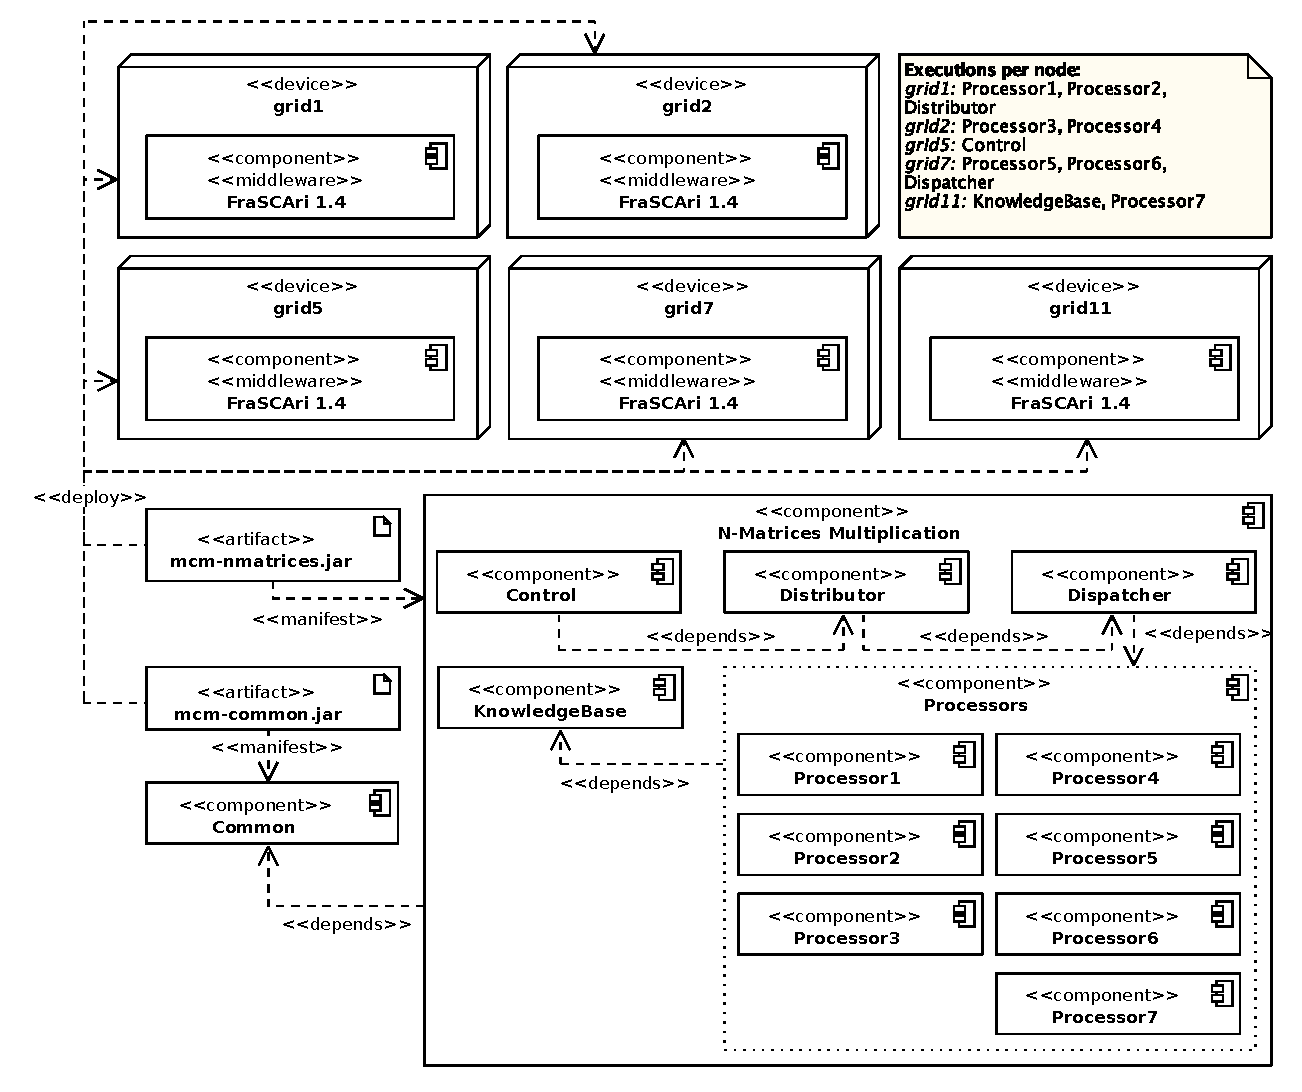
\includegraphics[width=0.8\textwidth]{fig/evaluation/nmatrices-deployment}
	\caption[]{Deployment Diagram for the N-Matrices Configuration Strategy}
	\label{fig:apx-eval-amelia-nmatrices}
\end{figure}
\end{comment}

\section{The \amelia{} Language: Specification Examples}

\amelia{} allows specifying two types of elements: Subsystems and Deployments. Along with this
practical guide you will be given an overview of the language syntax and the associated semantics. The following examples describe two deployment requirements and their corresponding solution in \amelia{}.

\subsection{Requirement 1 (Example)}
\label{subsect:apx-amelia-example-1}

Specify the deployment of the BlockReduce and Hybrid strategies having into account component dependencies and the computing nodes specified in the deployment diagram. You may use the following file containing a mapping between the hosts in the deployment diagrams and the laboratory's computers. \\

\begin{lstlisting}[style=common,caption=hosts.txt]
hgrid1	21	22	root	liasondriso_hgrid1	grid0
hgrid17	21	22	root	liasondriso_hgrid2	grid1
hgrid16	21	22	root	liasondriso_hgrid3	grid2
hgrid15	21	22	root	liasondriso_hgrid4	grid3
hgrid12	21	22	root	liasondriso_hgrid5	grid4
hgrid9	21	22	root	liasondriso_hgrid6	grid5
hgrid6	21	22	root	liasondriso_hgrid7	grid6
hgrid10	21	22	root	liasondriso_hgrid10	grid7
\end{lstlisting}



%In \amelia{} this would require to specify a \texttt{subsystem} for generating the corresponding artifacts from the Strassen and Common components' source code. Once they are generated, the Strassen component would be executed.

\subsubsection{Reusing code with \amelia{}}

In order to reduce the size of the deployment specifications with \amelia{} and promote reuse and maintainability concerns, we should begin the specification process through the identification and definition of elements that could be used repeatedly over this process. In case, we created a subsystem called \textit{Common}, which contains common definitions for all of the deployments/subsystems. \\   


\begin{lstlisting}[style=amelia,caption=Subsystem \textit{Common} for reusable definitions.]
package co.edu.icesi.driso.matrices

import java.util.List
import java.util.Map
import org.amelia.dsl.lib.descriptors.Host

/*
 * Common definitions for all of the deployments/subsystems.
 */
subsystem Common {

	/*
	 * All hosts.
	 */
	param Map<String, Host> hosts

	//-------------------------------------------------------------------------
	// Compilation parameters
	//-------------------------------------------------------------------------

	/*
	 * Compilation host.
	 */
	var Host compilationHost = hosts.get("grid0");

	/*
	 * Sources to compile.
	 */
	var String commonSources = "/home/sas1/LF_RIVERA/workspace-matrices/org.driso.matrices.common";
	var String blockRSources = "/home/sas1/LF_RIVERA/workspace-matrices/org.driso.matrices.blockreduce";
	var String hybridSources = "/home/sas1/LF_RIVERA/workspace-matrices/"
	+ "org.driso.matrices.hybrid_multiplication";
	var String nMatricesSources = "/home/sas1/LF_RIVERA/workspace-matrices/org.driso.matrices.nmatrices";
	var String strassenSources = "/home/sas1/LF_RIVERA/workspace-matrices/org.driso.matrices.strassen";

	/*
	 * Compilation sources.
	 */
	var List<String> sources = #[
        commonSources, blockRSources, hybridSources, nMatricesSources,
        strassenSources
	]

	/*
	 * Built sources folder (The site where compilation artifacts are located).
	 */
	var String builtFolder = "/home/sas1/LF_RIVERA/workspace-matrices/built-sources";

	//-------------------------------------------------------------------------
	// Allocation parameters
	//-------------------------------------------------------------------------

	/*
	 * The folder in the execution nodes where artifacts are allocated.
	 */
	var String allocationTargetFolder = "/home/sas1/";

	/*
	 * Target sources folder in the execution nodes
	 * (The site where the jars are executed).
	 */
	var String builtsFolder = '«allocationTargetFolder»built-sources';
}

\end{lstlisting}

As you probably noted, \amelia{} allows string interpolation through the use of guillemet symbols (\guillemotleft\guillemotright) between single quotation marks. Since string interpolation makes reading code much easier, especially when the string is part of a command declaration, string interpolations should be used instead of string concatenation. 

\subsubsection{Compiling sources with \amelia{}}

Since the addressed problem comprises multiple deployment strategies, we must compile certain software project sources for generating the desired specific artifacts to be deployed. In contemplation of standardization, we define a Java Enum for defining the possible deployment configurations for the matrix-chain multiplication problem. \\

\begin{lstlisting}[style=amelia,caption=Java Enum for possible deployment configurations.]
package co.edu.icesi.driso.matrices.classes;

/**
 * The mcm strategies.
 * @author Miguel Jimenez (miguel@uvic.ca)
 * @date 2017-08-19
 * @version $Id$
 * @since 0.0.1
 */
public enum Strategy {
    BLOCK_REDUCE,
    HYBRID_MULTIPLICATION,
    N_MATRICES,
    STRASSEN
}

\end{lstlisting}

We defined a subsystem called \textit{Compile} for the compilation of the associated source projects. This subsystem has a parameter for indicating the desired deployment strategy to be compiled. When defining the compilation subsystem, we can include the \textit{Common} subsystem that we have created previously through the clause \textit{includes}. All of the variables and rules defined in the \textit{Common} subsystem can be reused in the new \textit{Compile} subsystem, either to declare new variables or for defining new rules. This allows to avoid duplicating code and promotes reusability and composability concerns. For sake of simplicity, once artifacts have been generated, we need to place them in a shared folder. Therefore, we need to specify a dependency between two rules in the subsystem (compilation and relocation). \amelia{} supports this through the use of a colon symbol (:) separating the rules, following a pattern like \textit{dependantRule}:\textit{ruleDependency}. \\

\begin{lstlisting}[style=amelia,caption=Subsystem \textit{Compile} for compiling the source code.]
package co.edu.icesi.driso.matrices

import co.edu.icesi.driso.matrices.classes.Strategy

includes co.edu.icesi.driso.matrices.Common

/*
 * Compile each strategy's source code.
 */
subsystem Compile {
    /*
    * The multiplication strategy to compile.
    */
	param Strategy strategy

	on compilationHost {	 
		compileCommon:
			cd sources.get(0)
			compile "src" "mcm-common"
			cmd 'yes | cp -f mcm-common.jar «builtFolder»/'
	}

	on compilationHost ? strategy == Strategy.BLOCK_REDUCE {
		strategy1: compileCommon;
			cd sources.get(1)
			compile "src" "mcm-blockreduce" -classpath '«builtFolder»/mcm-common.jar'
			cmd 'yes | cp -f mcm-blockreduce.jar «builtFolder»'
	}

	on compilationHost ? strategy == Strategy.HYBRID_MULTIPLICATION {
		strategy2: compileCommon;
			cd sources.get(2)
			compile "src" "mcm-hybrid-multiplication" -classpath '«builtFolder»/mcm-common.jar'
			cmd 'yes | cp -f mcm-hybrid-multiplication.jar «builtFolder»'
	}

	on compilationHost ? strategy == Strategy.N_MATRICES {
		strategy3: compileCommon;
			cd sources.get(3)
			compile "src" "mcm-nmatrices" -classpath '«builtFolder»/mcm-common.jar'
			cmd 'yes | cp -f mcm-nmatrices.jar «builtFolder»'
	}

	on compilationHost ? strategy == Strategy.STRASSEN {
		strategy4: compileCommon;
			cd sources.get(4)
			compile "src" "mcm-strassen" -classpath '«builtFolder»/mcm-common.jar'
			cmd 'yes | cp -f mcm-strassen.jar «builtFolder»'
	}

}

\end{lstlisting}

\subsubsection{Artifacts transportation with \amelia{}}

Once artifacts have been generated from source code, they need to be transported (along with dependency libraries) to the computing nodes where they will be deployed. \amelia{} supports this requirement through the use of a command called \textit{scp}, nevertheless, in order to work, this command requires the configuration of an FTP Server. For sake of simplicity, we decided to exploit the extensibility of \amelia{} and created a new user-defined command that leverage the SSH-based secure copy command of Linux. For this purpose, we created a new class which contains a method for describing the user-defined \amelia{} command. \\

\begin{lstlisting}[style=amelia,caption=Class for defining a user-defined \amelia{} command.]
package co.edu.icesi.driso.matrices.classes;

import java.io.IOException;
import org.amelia.dsl.lib.CallableTask;
import org.amelia.dsl.lib.descriptors.CommandDescriptor;
import org.amelia.dsl.lib.descriptors.Host;
import net.sf.expectit.Expect;
import net.sf.expectit.matcher.Matchers;

public class SCPLogin {

	public static CommandDescriptor scpCommand(final String hostName,
	    final String hostPassword, final String source, final String target) {
		return new CommandDescriptor.Builder()
		    .withSuccessMessage("Copied file!")
			.withErrorMessage("File couldn't be copied!")
			.withCallable(new CallableTask<Object>() {
				@Override
				public Boolean call(Host host, String prompt, boolean quiet)
				    throws Exception {
					final Expect session = host.ssh().expect();
					session.sendLine(
					    String.format(
					        "scp -r root@%s:%s %s",
					        hostName,
					        source,
					        target
					    )
					);
					try {
						session.expect(
						    Matchers.regexp("Are you sure you want to continue connecting (yes/no)?")
						);
						session.sendLine("yes");
					} catch (IOException e) {
					    // Do nothing
					}
					session.expect(
					    Matchers.regexp(
					        String.format(
					            "root@%s's password:",
					            hostName
					        )
					    )
					);
					session.sendLine(hostPassword);
					session.expect(Matchers.regexp(prompt));
					return true;
				}
			}).build();
	}

}

\end{lstlisting}

With that in mind, we proceed to define a subsystem called \textit{Allocation} that allows the transportation of compiled artifacts and dependency libraries to the computing nodes where they will be deployed, i.e., the subsystem allocates software artifacts to executing computing nodes. This subsystem uses the user-defined command described previously. Transportation would not be possible if compilation was not successful. \amelia{} allows to model this requirement through the specification of dependencies between subsystems and rules. For dependencies between subsystems, it is necessary to specify the \textit{depends on} clause in conjunction with the subsystem in need for indicating that the dependant subsystem would not instantiated until its dependencies complete their execution. \\

\begin{lstlisting}[style=amelia,caption=Subsystem for artifacts allocation to computing nodes.]
package co.edu.icesi.driso.matrices

import co.edu.icesi.driso.matrices.classes.SCPLogin
import java.util.List
import org.amelia.dsl.lib.descriptors.Host

includes co.edu.icesi.driso.matrices.Common

depends on co.edu.icesi.driso.matrices.Compile

subsystem Allocation {

	param List<Host> executionHosts

	on executionHosts {
		move:
			SCPLogin.scpCommand(
	           compilationHost.hostname,
	           compilationHost.password,
	           builtFolder,
	           allocationTargetFolder
			)
	}
	
}
\end{lstlisting}

Once we granted the compilation and transportation of artifacts to the computing nodes that will execute them, we proceed to define two subsystems called \textit{BlockReduce} and \textit{Hybrid} that will execute their associated strategy. \\

\subsubsection{Execution of BlockReduce strategy}

\begin{lstlisting}[style=amelia,caption=Subsystem for executing BlockReduce strategy.]
package co.edu.icesi.driso.matrices

import java.util.List
import org.amelia.dsl.lib.descriptors.Host

includes co.edu.icesi.driso.matrices.Common

depends on co.edu.icesi.driso.matrices.Allocation

/*
 * Execute the BlockReduce multiplication strategy.
 */
subsystem BlockReduce {
	
	param List<Host> executionHosts
	
	var String common = "mcm-common"
	var String artifact = "mcm-blockreduce"
	var Iterable<String> libpath = #[
	 '«builtsFolder»/«common».jar',
	 '«builtsFolder»/«artifact».jar'
	]
	
	on executionHosts {
		init:
            cd builtsFolder
	}
	
	on hosts.get("grid1") {
		reducer0: matrixBuilder;
			run "BlocksMultiplicator0" -libpath libpath

		control: reducer0, reducer1, reducer2, reducer3, reducer4, reducer5;
			run "Blockreduce" -libpath libpath
	}
	
	on hosts.get("grid2") {
		reducer1: matrixBuilder;
			run "BlocksMultiplicator1" -libpath libpath
	}
	
	on hosts.get("grid3") {
		reducer2: matrixBuilder;
			run "BlocksMultiplicator2" -libpath libpath
	}
	
	on hosts.get("grid4") {
		reducer3: matrixBuilder;
			run "BlocksMultiplicator3" -libpath libpath
	}
	
	on hosts.get("grid5") {
		matrixBuilder: init;
			run "FinalMatrixBuilder" -libpath libpath
	
		reducer4: matrixBuilder;
			run "BlocksMultiplicator4" -libpath libpath
	}
	
	on hosts.get("grid6") {	
		reducer5: matrixBuilder;
			run "BlocksMultiplicator5" -libpath libpath
	}

}
\end{lstlisting}

\subsubsection{Execution of Hybrid strategy}

\begin{lstlisting}[style=amelia,caption=Subsystem for executing Hybrid strategy.]
package co.edu.icesi.driso.matrices

includes co.edu.icesi.driso.matrices.Common

depends on co.edu.icesi.driso.matrices.Allocation

/*
 * Execute the Hybrid multiplication strategy.
 */
subsystem HybridMultiplication {
	
	var String common = "mcm-common"
	var String artifact = "mcm-hybrid-multiplication"
	var Iterable<String> libpath = #[
        '«builtsFolder»/«artifact».jar',
        '«builtsFolder»/«common».jar'
	]

    on hosts.get("grid5") {
        reducer0:
			run "BlocksMultiplicator0" -libpath libpath

        reducer1:
			run "BlocksMultiplicator1" -libpath libpath

        control: reducer0, reducer1, reducer2, reducer3, reducer4, reducer5;
			run "HybridMultiplication" -libpath libpath
	}
	
	on hosts.get("grid3") {
		reducer2:
			run "BlocksMultiplicator2" -libpath libpath
	}
	
	on hosts.get("grid7") {
		reducer3:
			run "BlocksMultiplicator3" -libpath libpath
	}
	
	on hosts.get("grid6") {
		reducer4:
			run "BlocksMultiplicator4" -libpath libpath
	}
	
	on hosts.get("grid4") {
		reducer5:
			run "BlocksMultiplicator5" -libpath libpath
	}
	
}
\end{lstlisting}

Finally, we proceed to define one custom deployment for each strategy to be deployed. The custom deployment includes the subsystems defined previously and contains control flow statements that execute the deployment of a set of subsystems in a particular way. \\

\subsubsection{Custom deployment for the BlockReduce strategy}

\begin{lstlisting}[style=amelia,caption=Custom deployment for BlockReduce strategy.]
package co.edu.icesi.driso.matrices.deployments

import co.edu.icesi.driso.matrices.classes.Strategy
import java.util.List
import java.util.Map
import org.amelia.dsl.lib.descriptors.Host
import org.amelia.dsl.lib.util.Hosts

includes co.edu.icesi.driso.matrices.Common
includes co.edu.icesi.driso.matrices.Compile
includes co.edu.icesi.driso.matrices.Allocation
includes co.edu.icesi.driso.matrices.BlockReduce

/*
 * Deploy the BlockReduce strategy once and then
 * stop the executed components.
 */
deployment SimpleBlockReduce {
	// Load all hosts and then filter
	val Map<String, Host> hosts = Hosts.hosts("hosts.txt").toMap[h|h.identifier]
	val List<Host> executionHosts = #[
	   hosts.get("grid1"), hosts.get("grid2"), hosts.get("grid3"),
	   hosts.get("grid4"), hosts.get("grid5"), hosts.get("grid6")
	]

	// Add subsystems to deploy
	add(new Common(hosts))
	add(new Compile(Strategy.BLOCK_REDUCE, hosts))
	add(new Allocation(executionHosts, hosts))
	add(new BlockReduce(executionHosts, hosts))

	// Deploy and then stop the executed components
	start(true)
}
\end{lstlisting}

\subsubsection{Custom deployment for the Hybrid strategy}

\begin{lstlisting}[style=amelia,caption=Custom deployment for Hybrid strategy.]
package co.edu.icesi.driso.matrices.deployments

import co.edu.icesi.driso.matrices.classes.Strategy
import java.util.List
import java.util.Map
import org.amelia.dsl.lib.descriptors.Host
import org.amelia.dsl.lib.util.Hosts

includes co.edu.icesi.driso.matrices.Common
includes co.edu.icesi.driso.matrices.Compile
includes co.edu.icesi.driso.matrices.Allocation
includes co.edu.icesi.driso.matrices.HybridMultiplication

/*
 * Deploy the HybridMultiplication strategy once and then
 * stop the executed components.
 */
deployment SimpleHybridMultiplication {	 
    // Load all hosts and then filter
    val Map<String, Host> hosts = Hosts.hosts("hosts.txt").toMap[h|h.identifier]
    val List<Host> executionHosts = #[
        hosts.get("grid3"), hosts.get("grid4"), hosts.get("grid5"),
        hosts.get("grid6"), hosts.get("grid7")
    ]

    // Add subsystems to deploy
    add(new Common(hosts))
    add(new Compile(Strategy.HYBRID_MULTIPLICATION, hosts))
    add(new Allocation(executionHosts, hosts))
    add(new HybridMultiplication(hosts))

    // Deploy and then stop the executed components
    start(true)
}
\end{lstlisting}

 
\begin{comment} 
 
\subsection{Requirement 2 (Example)}

Specify the deployment of the Strassen strategy having into account component dependencies and the computing nodes specified in the deployment diagram. The deployment must be repeated ten times sequentially and retry on failure. \\

In this case we can reuse the specifications from Example \ref{subsect:apx-amelia-example-1} and specify only a custom deployment strategy that meets the requirement. The sequential deployments can be achieved using a \texttt{for} statement, and the retry-on-failure feature can be implemented using the \texttt{RetryableDeployment} utility class. \\

\end{comment}


\bibliographystyle{plain}
\bibliography{References}

\end{document}